% !TeX program = xelatex
\ifdefined\BookMaster\else
\documentclass[11pt,oneside]{article}
% !TeX program = xelatex
\usepackage[b5paper,left=22mm,right=22mm,top=20mm,bottom=22mm,footskip=11mm]{geometry}
\usepackage{fontspec}
\setmainfont{TeX Gyre Termes}
\setsansfont{TeX Gyre Heros}
\usepackage{amsmath,amssymb,mathtools,amsthm}
\renewcommand{\cdots}{\mathinner{\cdotp\cdotp\cdotp}}
\usepackage{graphicx,adjustbox,array,booktabs,longtable,multirow,enumitem,changepage,needspace}
\usepackage[table]{xcolor}
\usepackage{fancyhdr}
\raggedbottom
\interfootnotelinepenalty=10000
\newcommand{\BookFootnote}[2]{\begingroup\renewcommand{\thefootnote}{\fnsymbol{footnote}}\footnote[#1]{#2}\endgroup}
\newcommand{\BookFootnoteMark}[1]{\begingroup\renewcommand{\thefootnote}{\fnsymbol{footnote}}\footnotemark[#1]\endgroup}
\newcommand{\BookFootnoteText}[2]{\begingroup\renewcommand{\thefootnote}{\fnsymbol{footnote}}\footnotetext[#1]{#2}\endgroup}
\newenvironment{BookFloat}[1]{\par\addvspace{.6\baselineskip}\noindent\def\BookFloatID{#1}\begin{minipage}{\linewidth}\phantomsection\label{bookfloat:#1:start}}{\phantomsection\label{bookfloat:\BookFloatID:end}\end{minipage}\par\addvspace{.6\baselineskip}}

\usepackage[unicode,hidelinks]{hyperref}
\pagestyle{fancy}
\fancyhf{}
\newcommand{\BookFooter}{}
\fancyfoot[L]{\parbox[b]{\dimexpr\textwidth-15mm}{\footnotesize\BookFooter}}
\fancyfoot[R]{\footnotesize\thepage}
\renewcommand{\headrulewidth}{0pt}
\renewcommand{\footrulewidth}{0pt}
\setlength{\parindent}{0pt}
\setlength{\parskip}{0.2em}
\setlength{\emergencystretch}{3em}
\setlist{nosep,leftmargin=1.7em,labelsep=.65em}
\newif\ifBookNarrative
\BookNarrativetrue
\newenvironment{BookBody}{\setlength{\parindent}{0pt}}{}
\newcommand{\BookStatement}[1]{\par\addvspace{.6\baselineskip}\noindent #1\enspace\ignorespaces}
\newcommand{\BookLabel}[1]{\par\addvspace{.6\baselineskip}\needspace{3\baselineskip}\noindent\textbf{#1}\quad\ignorespaces}
\newcommand{\BookHeading}[1]{\par\addvspace{\baselineskip}\needspace{4\baselineskip}\noindent{\large\bfseries #1}\par\medskip}
\newcommand{\BookSubheading}[1]{\par\addvspace{.7\baselineskip}\needspace{3\baselineskip}\noindent{\bfseries #1}\par\smallskip}
\newcommand{\BookTextHeading}[1]{\par\addvspace{.7\baselineskip}\needspace{3\baselineskip}\noindent #1\par\smallskip}
\newcommand{\BookSectionTitle}[2]{\par\addvspace{1.2\baselineskip}\needspace{5\baselineskip}\noindent\colorbox{gray!25}{\sffamily\bfseries\small SECTION #1}\quad{\large\bfseries #2}\par\medskip}
\newcommand{\BookExerciseTitle}[1]{\par\addvspace{\baselineskip}\needspace{4\baselineskip}\noindent{\color{gray}\rule{1.5mm}{1.5mm}}\enspace{\large\bfseries Exercises #1}\par\medskip}
\newcommand{\BookBullet}[1]{\begin{list}{\textbullet}{\setlength{\leftmargin}{1.7em}\setlength{\labelwidth}{1em}\setlength{\labelsep}{.7em}\setlength{\topsep}{0pt}\setlength{\parsep}{0pt}\setlength{\itemsep}{0pt}}\item #1\end{list}}
\newcommand{\BookExercise}[2]{\begin{list}{\textbf{#1}}{\setlength{\leftmargin}{2.2em}\setlength{\labelwidth}{1.5em}\setlength{\labelsep}{.7em}\setlength{\topsep}{.15em}\setlength{\parsep}{0pt}\setlength{\itemsep}{0pt}}\item #2\end{list}}
\newcommand{\BookEnd}[1]{\unskip\nobreak\hfill\ensuremath{#1}}
\newcommand{\BookSource}[2]{\phantomsection\label{sourcepage:#1}} % Source-page anchors, retained through reflow.
\usepackage{multicol}
\usepackage{tikz}
\newcommand{\BookPartEntry}[2]{\par\noindent\makebox[17mm][l]{\bfseries Section #1}#2\par}
\newcommand{\BookPartTitle}[3]{\par\bigskip\noindent\begin{tikzpicture}\node[anchor=north west,inner sep=0pt,outer sep=0pt] (bookpart) at (0,0) {\begin{minipage}{\dimexpr\linewidth-.5pt}\hspace*{26mm}\begin{minipage}[t]{\dimexpr\linewidth-26mm}\begin{adjustbox}{max width=\linewidth}{\fontsize{20}{24}\selectfont\bfseries #2}\end{adjustbox}\par\vspace{6mm}\hrule\vspace{6mm}{\sffamily\footnotesize\setlength{\parskip}{.3em}#3}\vspace{3mm}\end{minipage}\end{minipage}};\path[shade,top color=gray!60,bottom color=white] (0,0) rectangle ([xshift=24mm]bookpart.south west);\node[anchor=north,font=\sffamily\bfseries\small] at (12mm,-2mm) {PART};\node[anchor=north,font=\sffamily\bfseries\Huge] at (12mm,-7mm) {#1};\end{tikzpicture}\par\bigskip}
\newsavebox{\BookMathBox}
\makeatletter
\newcommand{\BookInline}[1]{\leavevmode\hskip0pt\relax\begingroup\in@{\begin}{#1}\ifin@\sbox{\BookMathBox}{\(#1\)}\ifdim\wd\BookMathBox>\dimexpr\linewidth-1em\relax\resizebox{\dimexpr\linewidth-1em\relax}{!}{\usebox{\BookMathBox}}\else\(#1\)\fi\else\in@{\left}{#1}\ifin@\sbox{\BookMathBox}{\(#1\)}\ifdim\wd\BookMathBox>\dimexpr\linewidth-1em\relax\resizebox{\dimexpr\linewidth-1em\relax}{!}{\usebox{\BookMathBox}}\else\(#1\)\fi\else\(#1\)\fi\fi\endgroup\hskip0pt\relax}
\makeatother
\DeclareMathOperator{\Aut}{Aut}
\DeclareMathOperator{\End}{End}
\DeclareMathOperator{\Hom}{Hom}
\DeclareMathOperator{\GF}{GF}
\DeclareMathOperator{\irr}{irr}
\DeclareMathOperator{\lt}{lt}
\DeclareMathOperator{\lp}{lp}
\providecommand{\textcircled}[1]{\textnormal{(#1)}}

\begin{document}
\fi
\renewcommand{\BookFooter}{Section 16 Isomorphism Theorems}
\pdfbookmark[0]{Section 16 Isomorphism Theorems}{16_isomorphism_theorems}
\ifdefined\BookMaster\else\setcounter{page}{145}\fi
% Source PDF page 162; original printed page 145
\BookSource{162}{145}
\BookPartTitle{IV}{Advanced Group Theory}{\BookPartEntry{16}{Isomorphism Theorems}
\BookPartEntry{17}{Sylow Theorems}
\BookPartEntry{18}{Series of Groups}
\BookPartEntry{19}{Free Abelian Groups}
\BookPartEntry{20}{Free Groups}
\BookPartEntry{21}{Group Presentations}}

\BookNarrativetrue

\begin{BookBody}

\BookSectionTitle{16}{Isomorphism Theorems}

\noindent There are several theorems concerning isomorphic factor groups that are known as the \textit{isomorphism theorems} of group theory. The first of these is Theorem 12.14, which we restate for easy reference. The theorem is diagrammed in Fig. 16.1.

\begin{BookFloat}{16_isomorphism_theorems-p162-11}
\begin{center}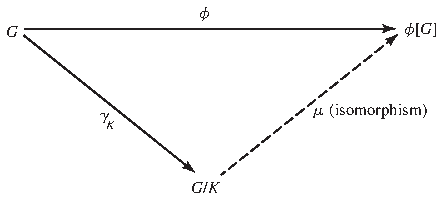
\includegraphics[width=0.604\linewidth,height=.8\textheight,keepaspectratio]{assets/p162_10.pdf}\end{center}
\begin{center}\small\textbf{16.1 Figure}\end{center}
\end{BookFloat}

\BookLabel{16.2 Theorem} \textbf{(First Isomorphism Theorem)} Let \BookInline{\phi:G\to G^{\prime }} be a homomorphism with kernel \BookInline{K,\allowbreak } and let \BookInline{\gamma _{K}:G\to G/K} be the canonical homomorphism. There is a unique isomorphism \BookInline{\mu:G/K\to \phi [G]} such that \BookInline{\phi (x)= \mu (\gamma _{K}(x))} for each \BookInline{x\in G.}\BookEnd{\blacklozenge}

The lemma that follows will be of great aid in our proof and intuitive understanding of the other two isomorphism theorems.

\BookLabel{16.3 Lemma} Let \BookInline{N} be a normal subgroup of a group \BookInline{G} and let \BookInline{\gamma:G\to G/N} be the canonical homomorphism. Then the map \BookInline{\phi } from the set of normal subgroups of \BookInline{G} containing \BookInline{N} to the set of normal subgroups of \BookInline{G/N} given by \BookInline{\phi (L)= \gamma [L]} is one-to-one and onto.

\BookLabel{\textit{Proof}} Theorem 13.18 shows that if \BookInline{L} is a normal subgroup of \BookInline{G} containing \BookInline{N,\allowbreak } then \BookInline{\phi (L)= } \BookInline{\gamma [L]} is a normal subgroup of \BookInline{G/N.} Because \BookInline{N\leq L,\allowbreak } for each \BookInline{x\in L} the entire coset \BookInline{xN} in \BookInline{G} is contained in \BookInline{L.} Thus by Theorem \BookInline{10.17,\allowbreak \gamma ^{- 1}[\phi (L)]= L.} Consequently, if \BookInline{L} and \BookInline{M} are normal subgroups of \BookInline{G,\allowbreak } both containing \BookInline{N,\allowbreak } and if \BookInline{\phi (L)= \phi (M)= H,\allowbreak } then \BookInline{L= \gamma ^{- 1}[H]= M.} Therefore \BookInline{\phi } is one-to-one.

\end{BookBody}

% Source PDF page 163; original printed page 146
\BookSource{163}{146}
\BookNarrativetrue

\begin{BookBody}

If \BookInline{H} is a normal subgroup of \BookInline{G/N,\allowbreak } then \BookInline{\gamma ^{- 1}[H]} is a normal subgroup of \BookInline{G} by Theorem 13.18. Because \BookInline{N\in H} and \BookInline{\gamma ^{- 1}[\{N\}]= N,\allowbreak } we see that \BookInline{N\subseteq \gamma ^{- 1}[H].} Then \BookInline{\phi (\gamma ^{- 1}[H])= \gamma [\gamma ^{- 1}[H]]= H.} This shows that \BookInline{\phi } is onto the set of normal subgroups of \BookInline{G/N.}\BookEnd{\blacklozenge}

If \BookInline{H} and \BookInline{N} are subgroups of a group \BookInline{G,\allowbreak } then we let

\begin{center}\begin{adjustbox}{max width=\linewidth}\BookInline{\displaystyle HN= \{hn\mid h\in H,\allowbreak n\in N\}.}\end{adjustbox}\end{center}

\noindent We define the\textbf{ join} \BookInline{H\vee N} of \BookInline{H} and \BookInline{N} as the intersection of all subgroups of \BookInline{G} that contain \BookInline{HN;} thus \BookInline{H\vee N} is the smallest subgroup of \BookInline{G} containing \BookInline{HN.} Of course \BookInline{H\vee N} is also the smallest subgroup of \BookInline{G} containing both \BookInline{H} and \BookInline{N,\allowbreak } since any such subgroup must contain \BookInline{HN.} In general\BookInline{,\allowbreak HN} need not be a subgroup of \BookInline{G.} However, we have the following lemma.

\BookLabel{16.4 Lemma} If \BookInline{N} is a normal subgroup of \BookInline{G,\allowbreak } and if \BookInline{H} is any subgroup of \BookInline{G,\allowbreak } then \BookInline{H\vee N= HN= } \BookInline{NH.} Furthermore, if \BookInline{H} is also normal in \BookInline{G,\allowbreak } then \BookInline{HN} is normal in \BookInline{G.}

\BookLabel{\textit{Proof}} We show that \BookInline{HN} is a subgroup of \BookInline{G,\allowbreak } from which \BookInline{H\vee N= HN} follows at once. Let \BookInline{h_{1},\allowbreak h_{2}\in H} and \BookInline{n_{1},\allowbreak n_{2}\in N.} Since \BookInline{N} is a normal subgroup, we have \BookInline{n_{1}h_{2}= h_{2}n_{3}} for some \BookInline{n_{3}\in N.} Then \BookInline{(h_{1}n_{1})(h_{2}n_{2})= h_{1}(n_{1}h_{2})n_{2}= h_{1}(h_{2}n_{3})n_{2}= (h_{1}h_{2})(n_{3}n_{2})\in HN,\allowbreak } so \BookInline{HN} is closed under the induced operation in \BookInline{G.} Clearly \BookInline{e= ee} is in \BookInline{HN.} For \BookInline{h\in H} and \BookInline{n\in N,\allowbreak } we have \BookInline{(hn)^{- 1}= n^{- 1}h^{- 1}= h^{- 1}n_{4}} for some \BookInline{n_{4}\in N,\allowbreak } since \BookInline{N} is a normal subgroup. Thus \BookInline{(hn)^{- 1}\in HN,\allowbreak } so \BookInline{HN\leq G.} A similar argument shows that \BookInline{NH} is a subgroup, so \BookInline{NH= H\vee N= HN.}

Now suppose that \BookInline{H} is also normal in \BookInline{G,\allowbreak } and let \BookInline{h\in H,\allowbreak n\in N,\allowbreak } and \BookInline{g\in G.} Then \BookInline{ghng^{- 1}= (ghg^{- 1})(gng^{- 1})\in HN,\allowbreak } so \BookInline{HN} is indeed normal in \BookInline{G.}\BookEnd{\blacklozenge}

We are now ready for the second isomorphism theorem.

\BookLabel{16.5 Theorem} \textbf{(Second Isomorphism Theorem)} Let \BookInline{H} be a subgroup of \BookInline{G} and let \BookInline{N} be a normal subgroup of \BookInline{G.} Then \BookInline{(HN)/N\simeq H/(H\cap N).}

\BookLabel{\textit{Proof}} Since \BookInline{N\leq HN\leq G} and \BookInline{N} is a normal subgroup of \BookInline{G,\allowbreak N} is a normal subgroup of \BookInline{HN,\allowbreak } which allows us to form the group \BookInline{HN/N.} We define a map \BookInline{\phi:H\to HN/N} by \BookInline{\phi (h)= hN.} The map \BookInline{\phi } is a homomorphism since for any \BookInline{h_{1},\allowbreak h_{2}\in H,\allowbreak }

\begin{center}\begin{adjustbox}{max width=\linewidth}\BookInline{\displaystyle \phi (h_{1}h_{2})= (h_{1}h_{2})N= (h_{1}N)(h_{2}N)= \phi (h_{1})\phi (h_{2}).}\end{adjustbox}\end{center}

\noindent The map \BookInline{\phi } maps onto \BookInline{HN/N} since any element of \BookInline{HN/N} can be written as \BookInline{hnN} for some \BookInline{h\in H} and \BookInline{n\in N} and \BookInline{hnN= hN= \phi (h).} We now compute the kernel of \BookInline{\phi.}

\begin{center}\begin{adjustbox}{max width=\linewidth}\BookInline{\displaystyle \;\text{Ker}\;(\phi )= \{h\in H\mid hN= N\}= \{h\in H\mid h\in N\}= H\cap N}\end{adjustbox}\end{center}

\noindent By the First Isomorphism Theorem, Theorem 16.2, the map \BookInline{\mu:H/(H\cap N)\to HN/N} defined by \BookInline{\mu (h(H\cap N))= hN} is an isomorphism\BookInline{.}\BookEnd{\blacklozenge}

\BookLabel{16.6 Example} Let \BookInline{G= \mathbb{Z}\times \mathbb{Z}\times \mathbb{Z},\allowbreak H= \mathbb{Z}\times \mathbb{Z}\times \{0\},\allowbreak } and \BookInline{N= \{0\}\times \mathbb{Z}\times \mathbb{Z}.} Then clearly \BookInline{HN= } \BookInline{\mathbb{Z}\times \mathbb{Z}\times \mathbb{Z}} and \BookInline{H\cap N= \{0\}\times \mathbb{Z}\times \{0\}.} We have \BookInline{(HN)/N\simeq \mathbb{Z}} and we also have \BookInline{H/(H\cap N)\simeq \mathbb{Z}.}\BookEnd{\blacktriangle}

\BookLabel{16.7 Example} Let \BookInline{G= \mathbb{Z},\allowbreak N= \langle n\rangle,\allowbreak } and \BookInline{H= \langle h\rangle } where \BookInline{n} and \BookInline{h} are positive. The group \BookInline{\mathbb{Z}} is abelian, so \BookInline{N} is a normal subgroup of \BookInline{Z.} Since \BookInline{\mathbb{Z}} is an additive group, we write \BookInline{N+ H} instead of \BookInline{NH} to avoid confusion. The group \BookInline{N+ H= \langle }gcd\BookInline{(n,\allowbreak h)\rangle } since anything in \BookInline{N+ H} is a multiple of gcd\BookInline{(n,\allowbreak h)} and gcd\BookInline{(n,\allowbreak h)= xn+ yh\in N+ H} for some integers \BookInline{x} and \BookInline{y.} Also\BookInline{,\allowbreak N\cap H= \langle }lcm\BookInline{(n,\allowbreak h)\rangle } since \BookInline{a\in N\cap H} if and only if \BookInline{a} is a multiple of both \BookInline{n} and \BookInline{h.} The Second Isomorphism Theorem states that \BookInline{(N+ H)/N= \langle }gcd\BookInline{(n,\allowbreak h)\rangle /\langle n\rangle } 
% Source PDF page 164; original printed page 147
\BookSource{164}{147}
is isomorphic with \BookInline{H/(N\cap H)= \langle h\rangle /\langle }lcm\BookInline{(n,\allowbreak h)\rangle.} In Exercise 10, you will be asked to prove that if \BookInline{a,\allowbreak b\in \mathbb{Z}^{+ }} and \BookInline{a} divides \BookInline{b,\allowbreak } then \BookInline{|\langle a\rangle /\langle b\rangle |= b/a.} Since \BookInline{\langle }gcd\BookInline{(n,\allowbreak h)\rangle /\langle n\rangle \simeq } \BookInline{\langle h\rangle /\langle }lcm\BookInline{(n,\allowbreak h)\rangle,\allowbreak } we have \BookInline{n\;\text{lcm}\;(n,\allowbreak h)}

\end{BookBody}

\BookNarrativetrue

\begin{BookBody}

\begin{center}\begin{adjustbox}{max width=\linewidth}\BookInline{\displaystyle \begin{aligned}\frac{n}{\gcd(n,\allowbreak  h)} &= \frac{\operatorname{lcm}(n,\allowbreak  h)}{h} \\nh &= \gcd(n,\allowbreak  h) \mathrm{lcm}(n,\allowbreak  h),\allowbreak \end{aligned}}\end{adjustbox}\end{center}

\noindent which provides a complicated way of proving a basic number theory fact! We conclude that

\begin{center}\begin{adjustbox}{max width=\linewidth}\BookInline{\displaystyle \langle \;\text{gcd}\;(n,\allowbreak h)\rangle /\langle n\rangle \simeq \langle h\rangle /\langle \;\text{lcm}\;(n,\allowbreak h)\rangle \simeq \mathbb{Z}_{\;\text{gcd}\;(n,\allowbreak h)}^{n}}\end{adjustbox}\end{center}

\noindent since a factor group of a cyclic group is cyclic. \BookEnd{\blacktriangle}

If \BookInline{H} and \BookInline{K} are two normal subgroups of \BookInline{G} and \BookInline{K\leq H,\allowbreak } then \BookInline{H/K} is a normal subgroup of \BookInline{G/K.} The third isomorphism theorem concerns these groups.

\BookLabel{16.8 Theorem} \textbf{(Third Isomorphism Theorem)} Let \BookInline{H} and \BookInline{K} be normal subgroups of a group \BookInline{G} with \BookInline{K\leq H.} Then \BookInline{G/H\simeq (G/K)/(H/K).}

\BookLabel{\textit{Proof}} Since \BookInline{K} is a subgroup of \BookInline{H,\allowbreak } for any \BookInline{g\in G,\allowbreak gK\subseteq gH.} That is, each left coset of \BookInline{K} is completely contained in one coset of \BookInline{H.} We define \BookInline{\phi:G/K\to G/H} by \BookInline{\phi (gK)= gH.} That is, we map a coset of \BookInline{K} to the coset of \BookInline{H} that contains it. Again, our strategy is to use the First Isomorphism Theorem. The map \BookInline{\phi } is a homomorphism since for any \BookInline{g_{1},\allowbreak g_{2}\in G,\allowbreak }

\begin{center}\begin{adjustbox}{max width=\linewidth}\BookInline{\displaystyle \begin{aligned}\phi ((g_{1}K)(g_{2}K))&= \phi ((g_{1}g_{2})K)= (g_{1}g_{2})H \\ &= (g_{1}H)(g_{2}H) \\ &= \phi (g_{1}K)\phi (g_{2}K).\end{aligned}}\end{adjustbox}\end{center}

\noindent The map \BookInline{\phi } maps onto \BookInline{G/H} since for any coset \BookInline{gH\in G/H,\allowbreak \phi (gK)= gH.} We now compute the kernel of \BookInline{\phi.}

\begin{center}\begin{adjustbox}{max width=\linewidth}\BookInline{\displaystyle \begin{aligned}\;\text{Ker}\;(\phi )&= \{gK\in G/K\mid gH= H\} \\ &= \{gK\in G/K\mid g\in H\} \\ &= H/K.\end{aligned}}\end{adjustbox}\end{center}

\noindent By the First Isomorphism Theorem \BookInline{(G/K)/(H/K)} is isomorphic with \BookInline{G/H} and a formula for an isomorphism \BookInline{\mu:(G/K)/(H/K)\to G/H} is \BookInline{\mu ((gK)H/K)= gH.}\BookEnd{\blacklozenge}

The formula for the isomorphism in the previous proof says that if we collapse the subgroup \BookInline{K} in \BookInline{G} to form \BookInline{G/K} and then collapse all the \BookInline{K} cosets inside of \BookInline{H} we have the same group as collapsing the subgroup \BookInline{H.} Figure 16.9 illustrates the situation. Think of the large ellipse as being the group \BookInline{G.} The cosets of \BookInline{H} are the sets bounded by the thick solid lines. The cosets of \BookInline{K} are the smaller sets inside the cosets of \BookInline{H.} The set \BookInline{G/H} consists of the cosets of \BookInline{H,\allowbreak } which are represented by the four larger areas, each of which is one point in \BookInline{G/H.} On the other hand\BookInline{,\allowbreak G/K} is represented by the twelve smaller sets each collapsed to a point. Then \BookInline{(G/K)/(H/K)} collapses each of the three small areas in the same \BookInline{H} coset to their common \BookInline{H} coset. Either way, we end up collapsing each \BookInline{H} coset to a point.

It is sometimes difficult to think about what groups look like when they contain more than one factor group in their definition. For example, what does an element of \BookInline{(G/K)/(H/K)} really look like? Keep in mind that a factor group has cosets of the subgroup as elements. Example 16.10 is intended to clarify what the group \BookInline{(G/K)/(H/K)} looks like and to explicitly show what the isomorphism of Theorem 16.8 looks like.

\end{BookBody}

% Source PDF page 165; original printed page 148
\BookSource{165}{148}
\BookNarrativetrue

\begin{BookBody}

\begin{BookFloat}{16_isomorphism_theorems-p165-0}
\begin{center}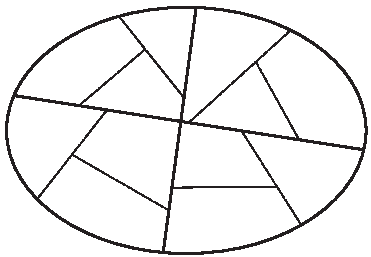
\includegraphics[width=0.509\linewidth,height=.8\textheight,keepaspectratio]{assets/p165_00.pdf}\end{center}
\begin{center}\small\textbf{16.9 Figure}\end{center}
\end{BookFloat}

\BookLabel{16.10 Example} Let \BookInline{G= \mathbb{Z}_{8},\allowbreak H= \langle 2\rangle = \{0,\allowbreak 2,\allowbreak 4,\allowbreak 6\}<G,\allowbreak } and \BookInline{K= \langle 4\rangle = \{0,\allowbreak 4\}<H.} We list the elements of each of the factor groups used in Theorem 16.8.

\begin{center}\begin{adjustbox}{max width=\linewidth}\BookInline{\displaystyle \begin{aligned}G/K&= \{\{0,\allowbreak 4\},\allowbreak \{1,\allowbreak 5\},\allowbreak \{2,\allowbreak 6\},\allowbreak \{3,\allowbreak 7\}\} \\ G/H&= \{\{0,\allowbreak 2,\allowbreak 4,\allowbreak 6\},\allowbreak \{1,\allowbreak 3,\allowbreak 5,\allowbreak 7\}\} \\ H/K&= \{\{0,\allowbreak 4\},\allowbreak \{2,\allowbreak 6\}\}\end{aligned}}\end{adjustbox}\end{center}

\noindent Before listing the elements of \BookInline{(G/K)/(H/K)} we note that any element of this group would be a coset of the subgroup \BookInline{H/K<G/K.} So each element is a set whose elements are sets.

\begin{center}\begin{adjustbox}{max width=\linewidth}\BookInline{\displaystyle (G/K)/(H/K)= \{\{\{0,\allowbreak 4\},\allowbreak \{2,\allowbreak 6\}\},\allowbreak \{\{1,\allowbreak 5\},\allowbreak \{3,\allowbreak 7\}\}\}}\end{adjustbox}\end{center}

\noindent Comparing \BookInline{G/H} and \BookInline{(G/K)/(H/K),\allowbreak } we see that each element in \BookInline{G/H} is the union of two cosets of \BookInline{K} in \BookInline{G/K.} Also, the isomorphism in Theorem 16.8 is the map \BookInline{\phi:} \BookInline{(G/K)/(H/K)\to G/H} defined by

\begin{center}\begin{adjustbox}{max width=\linewidth}\BookInline{\displaystyle \begin{aligned}\phi (\{\{0,\allowbreak 4\},\allowbreak \{2,\allowbreak 6\}\})&= \{0,\allowbreak 4,\allowbreak 2,\allowbreak 6\}\;\text{and}\; \\ \phi (\{\{1,\allowbreak 5\},\allowbreak \{3,\allowbreak 7\}\})&= \{1,\allowbreak 5,\allowbreak 3,\allowbreak 7\}.\end{aligned}}\end{adjustbox}\end{center}

\noindent So as illustrated in Figure 16.9, collapsing \BookInline{H} to form \BookInline{G/H} can be accomplished by first collapsing \BookInline{K} and then collapsing \BookInline{H/K.}\BookEnd{\blacktriangle}

\end{BookBody}

\BookNarrativefalse

\begin{BookBody}

\BookExerciseTitle{16}

\BookTextHeading{\textbf{Computations}}

\noindent In using the three isomorphism theorems, it is often necessary to know the actual correspondence given by the isomorphism and not just the fact that the groups are isomorphic. The first six exercises give us training for this.

\BookExercise{1.}{Let \BookInline{\phi:\mathbb{Z}_{12}\to \mathbb{Z}_{3}} be the homomorphism such that \BookInline{\phi (1)= 2.}}

\BookExercise{a.}{Find the kernel \BookInline{K} of \BookInline{\phi.}}

\BookExercise{b.}{List the cosets in \BookInline{\mathbb{Z}_{12}/K,\allowbreak } showing the elements in each coset.}

\BookExercise{c.}{Give the correspondence between \BookInline{\mathbb{Z}_{12}/K} and \BookInline{\mathbb{Z}_{3}} given by the map \BookInline{\mu } described in Theorem 16.2.}

\BookExercise{2.}{Let \BookInline{\phi:\mathbb{Z}_{18}\to \mathbb{Z}_{12}} be the homomorphism where \BookInline{\phi (1)= 10.}}

\BookExercise{a.}{Find the kernel \BookInline{K} of \BookInline{\phi.}}

\BookExercise{b.}{List the cosets in \BookInline{\mathbb{Z}_{18}/K,\allowbreak } showing the elements in each coset.}

\BookExercise{c.}{Find the group \BookInline{\phi [\mathbb{Z}_{18}].}}

\BookExercise{d.}{Give the correspondence between \BookInline{\mathbb{Z}_{18}/K} and \BookInline{\phi [\mathbb{Z}_{18}]} given by the map \BookInline{\mu } described in Theorem 16.2.}

\end{BookBody}

% Continuation on source PDF page 166, preceding Section 17
\BookNarrativefalse

\begin{BookBody}

\BookExercise{3.}{In the group \BookInline{\mathbb{Z}_{24},\allowbreak } let \BookInline{H= \langle 4\rangle } and \BookInline{N= \langle 6\rangle.}}

\BookExercise{a.}{List the elements in \BookInline{HN(}which we might write \BookInline{H+ N} for these additive groups) and in \BookInline{H\cap N.}}

\BookExercise{b.}{List the cosets in \BookInline{HN/N,\allowbreak } showing the elements in each coset.}

\BookExercise{c.}{List the cosets in \BookInline{H/(H\cap N),\allowbreak } showing the elements in each coset.}

\BookExercise{d.}{Give the correspondence between \BookInline{H/(H\cap N)} and \BookInline{HN/N} described in the proof of Theorem 16.5.}

\BookExercise{4.}{Repeat Exercise 3 for the dihedral group \BookInline{D_{6}} with \BookInline{N= \{\iota,\allowbreak \mu,\allowbreak \rho ^{2},\allowbreak \mu \rho ^{2},\allowbreak \rho ^{4},\allowbreak \mu \rho ^{4}\}} and \BookInline{H= \langle \rho \rangle.}}

\BookExercise{5.}{In the group \BookInline{G= \mathbb{Z}_{24},\allowbreak } let \BookInline{H= \langle 4\rangle } and \BookInline{K= \langle 8\rangle.}}

\BookExercise{a.}{List the cosets in \BookInline{G/H,\allowbreak } showing the elements in each coset.}

\BookExercise{b.}{List the cosets in \BookInline{G/K,\allowbreak } showing the elements in each coset.}

\BookExercise{c.}{List the cosets in \BookInline{H/K,\allowbreak } showing the elements in each coset.}

\BookExercise{d.}{List the cosets in \BookInline{(G/K)/(H/K),\allowbreak } showing the elements in each coset.}

\BookExercise{e.}{Give the correspondence between \BookInline{(G/K)/(H/K)} and \BookInline{G/H} described in the proof of Theorem 16.8.}

\BookExercise{6.}{Repeat Exercise 5 for the dihedral group \BookInline{G= D_{8},\allowbreak H= \langle \rho ^{2}\rangle = \{\iota,\allowbreak \rho ^{2},\allowbreak \rho ^{4},\allowbreak \rho ^{6}\},\allowbreak } and \BookInline{K= \langle \rho ^{4}\rangle = \{\iota,\allowbreak \rho ^{4}\}.}}

\BookTextHeading{\textbf{Theory}}

\BookExercise{7.}{Show directly from the definition of a normal subgroup that if \BookInline{H} and \BookInline{N} are subgroups of a group \BookInline{G,\allowbreak } and \BookInline{N} is normal in \BookInline{G,\allowbreak } then \BookInline{H\cap N} is normal in \BookInline{H.}}

\BookExercise{8.}{Let \BookInline{H,\allowbreak K,\allowbreak } and \BookInline{L} be normal subgroups of \BookInline{G} with \BookInline{H<K<L.} Let \BookInline{A= G/H,\allowbreak B= K/H,\allowbreak } and \BookInline{C= L/H.}}

\BookExercise{a.}{Show that \BookInline{B} and \BookInline{C} are normal subgroups of \BookInline{A,\allowbreak } and \BookInline{B<C.}}

\BookExercise{b.}{To what factor group of \BookInline{G} is \BookInline{(A/B)/(C/B)} isomorphic?}

\BookExercise{9.}{Let \BookInline{K} and \BookInline{L} be normal subgroups of \BookInline{G} with \BookInline{K\vee L= G,\allowbreak } and \BookInline{K\cap L= \{e\}.} Show that \BookInline{G/K\simeq L} and \BookInline{G/L\simeq K.}}

\BookExercise{10.}{Use one of the Isomorphism Theorems to prove that if \BookInline{a,\allowbreak b\in \mathbb{Z}^{+ }} and \BookInline{a} divides \BookInline{b,\allowbreak } then \BookInline{|a\mathbb{Z}/b\mathbb{Z}|= b/a.}}

\BookExercise{11.}{Let \BookInline{G} be a group with subgroups \BookInline{H^{\ast }\leq H\leq G} and \BookInline{K^{\ast }\leq K\leq G.} Prove that the sets \BookInline{H^{\ast }(H\cap K^{\ast })\cap (H\cap K)} and \BookInline{(H^{\ast }\cap K)(H\cap K^{\ast })} are equal.}

\end{BookBody}
\ifdefined\BookMaster\let\BookFinish\relax\else\def\BookFinish{\end{document}}\fi\BookFinish
